\documentclass[UTF8,a4paper,12pt]{ctexbook} 

\usepackage{graphicx}%学习插入图
\usepackage{verbatim}%学习注释多行
\usepackage{booktabs}%表格
\usepackage{geometry}%图片
\usepackage{amsmath}
\usepackage{amssymb}
\usepackage{listings}%代码
\usepackage{xcolor}  %颜色
\usepackage{enumitem}%列表格式
\setenumerate[1]{itemsep=0pt,partopsep=0pt,parsep=\parskip,topsep=5pt}
\setitemize[1]{itemsep=0pt,partopsep=0pt,parsep=\parskip,topsep=5pt}
\setdescription{itemsep=0pt,partopsep=0pt,parsep=\parskip,topsep=5pt}
\usepackage{tcolorbox}
\usepackage{algorithm}  %format of the algorithm
\usepackage{algorithmic}%format of the algorithm
\usepackage{multirow}   %multirow for format of table
\usepackage{tabularx} 	%表格排版格式控制
\usepackage{array}	%表格排版格式控制
\usepackage{hyperref} %超链接 \url{URL}
\usepackage{dirtree}
\setmainfont{Times New Roman}
\graphicspath{{figure/}}
\CTEXsetup[format+={\flushleft}]{section}
%%%% 段落首行缩进两个字 %%%%
\makeatletter
\let\@afterindentfalse\@afterindenttrue
\@afterindenttrue
\makeatother
\setlength{\parindent}{2em}  %中文缩进两个汉字位

%%%% 下面的命令重定义页面边距,使其符合中文刊物习惯 %%%%
\addtolength{\topmargin}{-54pt}
\setlength{\oddsidemargin}{0.63cm}  % 3.17cm - 1 inch
\setlength{\evensidemargin}{\oddsidemargin}
\setlength{\textwidth}{14.66cm}
\setlength{\textheight}{24.00cm}    % 24.62

%%%% 下面的命令设置行间距与段落间距 %%%%
\linespread{1.4}
\setlength{\parskip}{0.5\baselineskip}
\geometry{left=1.6cm,right=1.8cm,top=2cm,bottom=1.7cm} %设置文章宽度
\pagestyle{plain} 		  %设置页面布局

%代码效果定义
\definecolor{mygreen}{rgb}{0,0.6,0}
\definecolor{mygray}{rgb}{0.5,0.5,0.5}
\definecolor{mymauve}{rgb}{0.58,0,0.82}
\lstset{ %
	backgroundcolor=\color{white},   % choose the background color
	basicstyle=\footnotesize\ttfamily,      % size of fonts used for the code
	%stringstyle=\color{codepurple},
	%basicstyle=\footnotesize,
	%breakatwhitespace=false,         
	%breaklines=true,                 
	%captionpos=b,                    
	%keepspaces=true,                 
	%numbers=left,                    
	%numbersep=5pt,                  
	%showspaces=false,                
	%showstringspaces=false,
	%showtabs=false,        
	columns=fullflexible,
	breaklines=true,                 % automatic line breaking only at whitespace
	captionpos=b,                    % sets the caption-position to bottom
	tabsize=4,
	commentstyle=\color{mygreen},    % comment style
	escapeinside={\%*}{*)},          % if you want to add LaTeX within your code
	keywordstyle=\color{blue},       % keyword style
	stringstyle=\color{mymauve}\ttfamily,     % string literal style
	frame=single,
	rulesepcolor=\color{red!20!green!20!blue!20},
	% identifierstyle=\color{red},
	language=c++,
}
 \author{\kaishu 郑华}
 \title{Shell 笔记}
 
\begin{document}          %正文排版开始
 	\maketitle
 	\tableofcontents

\chapter{Bash 基本功能}
	\section{基本}
		\paragraph{history}查看历史命令
			\begin{itemize}
				\item \verb|-c :|清空历史命令
				\item \verb|-w :|把缓存中的历史命令写入历史命令保存文件\verb|~/.bash_history|
			\end{itemize}
			
			历史命令默认保存条数可以在文件\verb|/etc/profile 中|进行设置
			
		\paragraph{alias}定义别名 \verb|alias 别名='原命令'|
		
			删除别名\verb|unalias|
		
		\paragraph{命令执行时顺序}
			\begin{enumerate}
				\item 首先执行用绝对路径或相对路径执行的命令
				\item 其次执行别名(alias)关联的命令
				\item 其次执行Bash 的内部命令
				\item 最后执行按照\verb|$PATH|环境变量定义的目录查找顺序找到的第一个命令
			\end{enumerate}
		
		\paragraph{Bash 快捷键}如表\ref{bash_k}所示:
			\begin{table}[H]
				\centering
				\caption{bash 快捷键}
				\label{bash_k}
				\begin{tabular}{p{2cm}<{\centering}|p{12cm}<{\centering}}
					\toprule[1.5pt]
					快捷键  &  作用含义\\
					\hline
					\verb|ctr+A | &  把光标移动到命令行开头   \\
					\verb|ctr+E | &  把光标移动到命令行结尾   \\
					\verb|ctr+C | &  强制终止当前命令   \\
					\verb|ctr+L | &  清屏,相当于clear 命令   \\
					\verb|ctr+U | &  剪切(dd)光标之前的命令   \\
					\verb|ctr+K | &  剪切光标之后的命令   \\
					\verb|ctr+Y | &  粘贴ctr+U或ctr+K剪切的内容   \\
					\verb|ctr+R | &  在历史命令中搜索   \\
					\verb|ctr+D | &  退出当前终端   \\
					\verb|ctr+Z | &  暂停,并放入后台   \\
					\verb|ctr+S | &  暂停屏幕输出   \\
					\verb|ctr+Q | &  恢复屏幕输出   \\
					\bottomrule[1.5pt]
				\end{tabular}
			\end{table}

		\paragraph{环境变量配置文件}为使得环境变量永久生效的文件,主要是定义对系统的操作环境生效的默认环境变量,比如\verb|PATH|、\verb|HISTSIZE|、\verb|PS1|、\verb|HOMENAME|等默认变量。
		
			保存在\verb|/etc/|目录下的配置文件是对所有用户都生效的。而保存在用户当前目录\verb|~/|则只对当前用户生效
		
			\subparagraph{环境变量叠加方式}\verb|PATH='$PATH':/root| 
				将\verb|/root|添加到环境变量中,但是这样更改后,下次重启会消失。如果想要长久生效需要更改配置文件。
			
			\subparagraph{执行顺序}执行过程如下所图\ref{env}示\verb|->|
				\begin{figure}[htb]
					\centering
					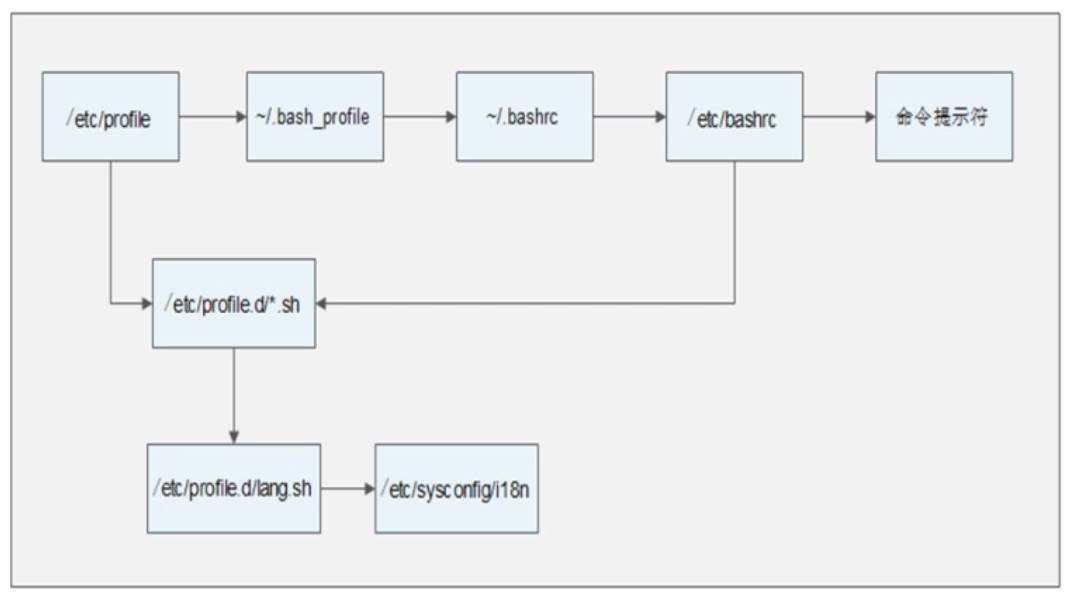
\includegraphics[scale=0.3]{env.png}
					\caption{执行顺序}
					\label{env}
				\end{figure}
				
			\subparagraph{/etc/profile}
				定义\verb|PATH、LOGNAME、HISTSIZE、HOSTNAME 等|,调用\verb|/etc/profile.d/|目录下的所有脚本文件.sh并执行。
				
				然后进入用户目录,调用\verb|~/.bash_profile|,追加\verb|PATH|并生效,并间接调用\verb|~/.bashrc|,完成别名定义, 并简介调用\verb|/etc/bashrc| 配置文件完成不用登陆的shell 配置并生效。
			
			\subparagraph{/etc/profile.d/*.sh}这部分脚本主要设置语言等
			
			\subparagraph{~/.bash\_profile}设置登陆用户的环境变量\verb|$PATH|, 并调用配置\verb|~/.bashrc|
			
			\subparagraph{~/.bashrc}设置登录用户的\textbf{别名设置}, 并调用配置\verb|/etc/bashrc|
			
			\subparagraph{/etc/bashrc}设置未登录的BASH 环境变量
			
		
		\paragraph{source}\verb|source 配置文件 => .  配置文件| 使配置文件生效。
	
	\section{字符截取}
		\dirtree{%		
			.1 字符截取.
			.2 截取行.
			.3 grep.
			.3 sed.
			.2 截取列.
			.3 cut.
			.3 awk.
		}
		\paragraph{grep}\verb|grep 选项 字符串 文件名|

		\paragraph{cut}\verb|cut 选项 文件名|,有局限,仅支持制表符、和常用分隔符(,:。-),不支持空格。
			\begin{itemize}
				\item \verb|-f列号 |提取第几列
				\item \verb|-d分隔符 |按照指定分隔符分割列
			\end{itemize}
			
			\verb|cut -f 2 student.txt| 提取文件第2列
			
			\verb|cut -f 2,3 student.txt| 提取文件第2列和第三列
			
			\verb|cut -d ":" -f 1,3 /etc/passwd| 截取第一列和第三列,并且分隔符号为:
	
	\section{awk}
		\subsection{基本使用}
			\paragraph{使用格式}
				\verb|awk '条件1{动作1} 条件2{动作2}...' 文件名|, 先读入一行,然后逐行执行操作。
				
				\subparagraph{条件 Pattern}一般使用关系表达式作为条件
					\begin{itemize}[itemindent = 1em]
						\item \verb|x > 10|
						\item \verb|x >= 10|
						\item \verb|x <= 10|
					\end{itemize}
			
				\subparagraph{动作 Action}
					\begin{itemize}[itemindent = 1em]
						\item 格式化输出
						\item 流程控制语句
					\end{itemize}
			
			\paragraph{例子}
				\begin{itemize}
					\item \verb|awk ' {printf $2 "\t" $6 "\n"}'   student.txt|  :patten 省略,表示对每行都执行,显式文件中的第2列和第6列。
					\item \verb@df -h|awk '{print $1 "\t" $3}' @: 截取df 输出的第1列和第三列, 与cut 不同的是,awk 无须指定分割符,并且需要注意的是,print 会自动分行,但是格式控制与printf 相同。
				\end{itemize}
				
		
		\subsection{awk 编程}
			\paragraph{使用格式}
				
				\subparagraph{BEGIN} 在其他所有命令逐行执行前,执行一次 BEGIN后的动作
				
					\verb|awk 'BEGIN{print "Test awk BEGIN"} {print $2 "\t" $5}'  student.txt|
					
					这条命令首先执行BEGIN 后的 print Anction, 然后逐行读取数据执行之后的条件与动作。
			
				\subparagraph{FS内置变量} 指定分隔符
				
					\verb|awk '{FS=":"}{print $1"\t"$3}'  /etc/passwd|
					
					这条命令意思是指定分割符为:,但是在读入第一行后,再执行后面Action 时,指定分隔符已经来不及了,所以这种情况第一行时不会正确使用分割符分割的,而是从第2行开始的,为了解决这个问题,可以利用前面提到的BEGIN 解决。
					
					\verb|awk 'BEGIN{FS=":"}{xx}'  xx|
				
				\subparagraph{END} 在所有命令执行完后,执行一次 END后的动作
					
					\verb|awk '{print $1"\t"$3}  END{print"The End"}'  student.txt|	
					
				
				\subparagraph{关系运算}
					\verb@cat fileName.txt | grep -v Name | awk '$6 >= 87 {print $2}'@

	\section{sed} 轻量\textbf{流}(与vi相比支持管道操作)编辑器,主要用来将数据进行选取、替换、删除、新增的命令。
	
		\paragraph{使用格式}
			\verb|sed [选项] '[动作]'  文件名|
			
			\begin{itemize}
				\item \verb|-n |一般sed 命令会将所有数据都输出到屏幕,而如果使用-n 选项,则只会将经过sed 命令处理的行输出到屏幕
				\item \verb|-e |允许对输入数据应用多条sed 命令编辑
				\item \verb|-i |用sed 的修改结果直接修改读取数据的文件,而不是由屏幕输出。
			\end{itemize}
			
		\paragraph{动作}
			\begin{itemize}
				\item \verb|a |追加,在当前行后添加一行或多行。 添加多行时,除最后一行外,每行末尾需要用\verb|“\”| 代表数据未完结。
				\item \verb|c |行替换,用c 后面的字符串替换原数据行,替换多行时,除最后一行外,每行末尾需用\verb|“\” |代表数据未完结。
				\item \verb|i |插入, 在当前行前插入一行或多行,插入多行...
				\item \verb|d |删除,删除指定行
				\item \verb|p |打印,输出指定行
				\item \verb|s |字符替换,用一个字符串替换另一个字符串。格式为\verb|"行范围s/旧字符串/新字符串/g"|
			\end{itemize}
  
  	
\chapter{Shell 基本知识}
		 \section{Shell}
			 \textbf{Shell就是一个命令行解释器},它的作用是解释执行用户的命令,用户输入一条命令,Shell就解释执行一条,这种方式称为交互式(Interactive)
			 
			 Shell还有一种执行命令的方式称为\textbf{批处理(Batch)},\textit{用户事先写一个Shell脚本(Script)},\textbf{其中有很多条命令,让Shell一次把这些命令执行完,而不必一条一条地敲 命令}。Shell脚本和编程语言很相似,也有变量和流程控制语句,包括循环和分支。但\textbf{Shell脚本是解释执行的,不需 要编译,Shell程序从脚本中一行一行读取并执行这些命令,相当于一个用户把脚本中的命令一行一 行敲到Shell提示符下执行}。作为程序设计语言,它虽然不是 Linux系统内核的一部分,但它调用了系统内核的大部分功能来执行程序、创建文档并以并行的方式协调各个程序的运行
		 \section{Shell 执行脚本}
			 shell执行脚本是一门解释性语言、批量化处理语言,大大的节省了工作成本,shell\textbf{脚本第一行必须以}\verb|#!|\textbf{开头},\textit{它表示该脚本使用后面的解释器解释执行}。
			 
			\subparagraph{Example:}
			 //script.sh   注:这是一个文本文件
			 \begin{lstlisting}[frame=L,xleftmargin=.06\textwidth]
	#!/bin/bash
	#注意 echo 默认为换行输出,如果不换行+\c 
	echo "this is a test"	
	ls
	ls -l
	echo "there are all files"
			 \end{lstlisting}
			 
			 \paragraph{执行方式}
				 \begin{lstlisting}[frame=L,xleftmargin=.06\textwidth]
	//第一种执行方式:
	[admin@localhost Shell]$ chmod +x  script.sh
	[admin@localhost Shell]$ ./script.sh
	
	//第二种执行方式:
	[admin@localhost Shell]$ /bin/bash  script.sh
	//等价于:
	[admin@localhost Shell]$ shell  script.sh
				 \end{lstlisting}
		 
			 \paragraph{执行过程}
				 Shel会fork一个子进程并调用exec执行./script.sh这个程序,exec系统调用应该把子进程的代码段替换成./script.sh程序的代码段,并从它的\_start始执行。然而script.sh是个文本文件,根 本没有代码段和\_start函数,怎么办呢?其实exec还有另外一种机制,如果要执行的是一个文本文件,并且第一行 指定了解释器,则用解释器程序的代码段替换当前进程,并且从解释器 的\_start开始执行,而这个文本文件被当作命令行参数传给解释器。因此,执行上述脚本相当于执行程序!
				 
				 什么是“子程序”呢?就是说,在我目前这个 shell 的情况下,去启用另一个新的 shell ,新的那个 shell 就是子程序
				 
				 这个程序概念与变量有啥关系啊?关系可大了!因为子程序仅会继承父程序的环境变量, 子程序不会继承父程序的自订变量
				 \begin{enumerate}
				 	\item 交互式进程(父进程)创建一个子进程用于执行脚本,父进程等待子进程终止
				 	\item 子进程程序替换bash解释器
				 	\item 读取shell脚本的命令,将其以参数传递的方式传递给bash解释器
				 	\item 子bash对shell脚本传入的参数进行读取,读一行识别到它是一个命令,则再创建一个子进程,子bash等待该新进程终止
				 	\item 新进程执行该命令,执行完后将结果交给子进程
				 	\item 子进程继续读取命令,创建新进程,新进程执行该命令,将结果返回给子进程,直到执行完最后一条命令
				 	\item 子进程终止,将结果返回给交互式父进程
				 \end{enumerate}
				 
				 \subparagraph{注意}注意:像export、cd、env、set 这些内置命令,在键入命令行后,交互式进程不会创建子进程,而是调用bash内部的函数执行这些命令,改变的是交互式进程。
				 
				 如果在命令行下,将多个命令用括号括起来,并用分号隔开来执行,交互式进程依然会创建一个子shell执行括号中的命令:
					 \begin{figure}[h]
					 	\begin{center}
						 	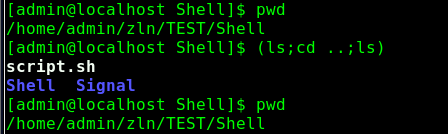
\includegraphics[scale = 0.5]{figure/ShellBracket.png}
						 	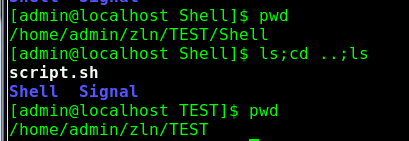
\includegraphics[scale = 0.5]{figure/ShellBracketNo.png}
						\end{center}
					 	\caption{(comands) VS Comands}
					 \end{figure}
				 
				 \textbf{\underline{.} 或者 \underline{source}这两个命令}是Shell的内建命令,\textbf{这种方式不会创建子Shell},\textbf{而是直接在交互式Shell下逐行 执行脚本中的命令}
				 
				 \subparagraph{Example}
					 \begin{lstlisting}[frame=L,xleftmargin=.06\textwidth]

#!/bin/bash
ls
echo "#################"
cd ..
ls
					 \end{lstlisting}
					 \begin{figure}[h]
					 	\centering
					 	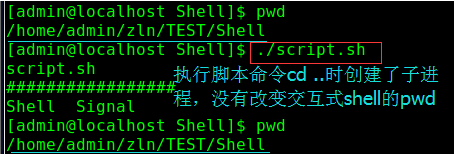
\includegraphics[scale = 0.5]{figure/SourceExample.png}
					 	\caption{without use . Or source Command}
					 \end{figure}
					 \begin{figure}[h]
					 	\begin{center}
					 		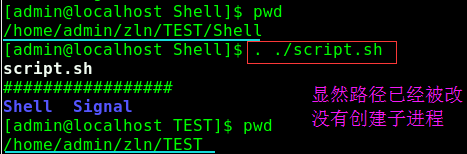
\includegraphics[scale = 0.5]{figure/SourceExample1.png}
					 		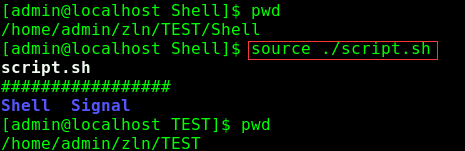
\includegraphics[scale = 0.5]{figure/SourceExample2.png}
					 	\end{center}
					 	\caption{Use . Or source Command}
					 \end{figure}
					 
				shell子进程:\url{https://blog.csdn.net/sosodream/article/details/5683515}
				
		 \section{Shell 变量}
			 shell变量不需要进行任何声明,直接定义即可,因为shell变量的值实际上都是字符串(对于没有定义的变量默认是一个空串)。定义的时候shell变量由大写字母加下划线组成,并且定义的时候等号两边不能存在空格,否则会被认为是命令!
			 
			 \paragraph{shell变量的种类}
				 \subparagraph{环境变量:}shell进程的环境变量可以从当前shell进程传给fork出来的子进程
				 \subparagraph{本地变量:}只存在于当前shell进程
				 
				 利用printenv可以显示当前shell进程的环境变量;利用set命令可以显示当前shell进程中的定义的所有变量(包括环境变量和本地变量)和函数。
				 
				 一个shell变量定义后仅存在于当前Shell进程,是一个本地变量。用export命令可以把本地变量导出为环境变量。用unset命令可以删除已定义的环境变量或本地变量。
					 \begin{lstlisting}[frame=L,xleftmargin=.06\textwidth]
	//分步  先定义后导出
	COUNT=5
	export COUNT
	
	//一步完成定义和导出环境变量
	export COUNT=5 
	
	//删除已经定义的环境变量
	unset COUNT
					 \end{lstlisting}
				
				\subparagraph{变量引用:}引用shell变量要用到\$符号,加\verb|{}|可以防止歧义。
					\begin{lstlisting}[frame=L,xleftmargin=.06\textwidth]
	COUNT=5
	echo $COUNT
	echo ${COUNT}911
					\end{lstlisting}
				
					\begin{figure}[h]
						\centering
						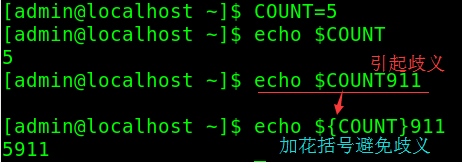
\includegraphics[scale = 0.7]{figure/ShellRefVariable.png}
						\caption{Shell Variable Use}
					\end{figure}
				\subparagraph{只读变量}
					使用 readonly 命令可以将变量定义为只读变量,只读变量的值不能被改变。
					
					下面的例子尝试更改只读变量,结果报错:
					\begin{lstlisting}[frame=L,xleftmargin=.06\textwidth]
	#!/bin/bash
	myUrl="http://www.w3cschool.cc"
	readonly myUrl
	myUrl="http://www.runoob.com"
	
	//运行脚本,结果如下:
	/bin/sh: NAME: This variable is read only.
					\end{lstlisting}
					
				\subparagraph{删除变量}
					使用 unset 命令可以删除变量。语法:unset variable\_name,变量被删除后不能再次使用。unset 命令不能删除只读变量。
					\begin{lstlisting}[frame=L,xleftmargin=.06\textwidth]
	#!/bin/sh
	myUrl="http://www.runoob.com"
	unset myUrl
	echo $myUrl
	
	// 以上没输出
					\end{lstlisting}
					
				\subparagraph{Shell 字符串}
					字符串是shell编程中最常用最有用的数据类型(除了数字和字符串,也没啥其它类型好用了),字符串可以用单引号,也可以用双引号,也可以不用引号。
					\begin{itemize}
						\item \textbf{单引号字符串的限制:}
							\begin{enumerate}
								\item 单引号里的任何字符都会原样输出,单引号字符串中的变量是无效的;
								\item 单引号字串中不能出现单引号(对单引号使用转义符后也不行)。
							\end{enumerate}
						
						\item \textbf{双引号字符串的好处:}
							\begin{enumerate}
								\item \textbf{双引号里可以有变量}
								\item \textbf{双引号里可以出现转义字符}
							\end{enumerate}
					\end{itemize}
					
					\begin{lstlisting}[xleftmargin=.06\textwidth]
	str='this is a string'
	your_name='qinjx'
	str="Hello, I know your are \"$your_name\"! \n"
	
	// 拼接字符串
	your_name="qinjx"
	greeting="hello, "$your_name" !"
	greeting_1="hello, ${your_name} !"
	echo $greeting $greeting_1
	
	// 获取字符串长度 
	string="abcd"
	echo ${#string} #输出 4
	
	// 提取子字符串:以下实例从字符串第 2 个字符开始截取 4 个字符
	string="runoob is a great site"
	echo ${string:1:4} # 输出 unoo
	
	// 查找子字符串:查找字符 "i 或 s" 的位置:
	string="runoob is a great company"
	echo 'expr index "${string}" is'  //# 输出 8
					\end{lstlisting}
					
				\subparagraph{Shell 数组}
					bash\textbf{支持一维数组}(不支持多维数组),并且没有限定数组的大小。
					类似与C语言,数组元素的下标由0开始编号。获取数组中的元素要利用下标,下标可以是整数或算术表达式,其值应大于或等于0
					\begin{itemize}
						\item  \textbf{定义数组}:用括号来表示数组,数组元素用"空格"符号分割开。定义数组的一般形式为:数组名=(值1 值2 ... 值n),还可以单独定义数组的各个分量
						 
						\item  \textbf{读取数组}:\verb|${数组名[下标]}|
						\item  \textbf{求数组长度}:获取数组长度的方法与获取字符串长度的方法相同,length=\verb|${#array_name[@]}|
					\end{itemize}
				
					\begin{lstlisting}[xleftmargin=.06\textwidth]
	// 定义数组
	array_name=(value0 value1 value2 value3)
	array_name=(
		value0
		value1
		value2
		value3
	)
	// 单独定义数组的各个分量
	array_name[0]=value0
	array_name[1]=value1
	array_name[n]=valuen
	
	// 读取数组各元素和所有元素
	valuei=${array_name[i]}
	// 使用@符号可以获取数组中的所有元素
	echo ${array_name[@]}
	
	// 获取数组的长度 
	# 取得数组元素的个数
	length=${#array_name[@]}
	# 或者
	length=${#array_name[*]}
	# 取得数组单个元素的长度
	lengthn=${#array_name[n]}
					\end{lstlisting}
				\subparagraph{Shell 注释}
					以\verb|#|开头的行为注释行
				
				
		 \section{Shell 通配符、命令代换、单引号、双引号}
			 见基础相关拓展.
	 
		 \section{Shell 传递参数}
			 我们可以在执行 Shell 脚本时,向脚本传递参数,脚本内获取参数的格式为:\verb|$n|。n 代表一个数字,1 为执行脚本的第一个参数,2 为执行脚本的第二个参数,以此类推……
			 
			 \begin{itemize}
			 	\item  \verb|$#|:参数个数
			 	\item  \verb|$$|:当前shell的PID进程ID
			 	\item  \verb|$@和$*|均表示所有参数,形式有所不同。\verb|$@:"$1" "$2" … "$n"|; \verb|$*: "$1 $2 … $n"|。
			 \end{itemize}
			 
			 \begin{lstlisting}[xleftmargin=.06\textwidth]
	//以下实例我们向脚本传递三个参数,并分别输出,其中 $0 为执行的文件名
	#!/bin/bash	
	echo "Shell 传递参数实例!";
	echo "执行的文件名:$0";
	echo "第一个参数为:$1";
	echo "第二个参数为:$2";
	echo "第三个参数为:$3";
	
	$ chmod +x test.sh 
	$ ./test.sh 1 2 3
	Shell 传递参数实例!
	执行的文件名:./test.sh
	第一个参数为:1
	第二个参数为:2
	第三个参数为:3
			 \end{lstlisting}
			 
		\section{Shell 各种括号}
			\url{http://blog.csdn.net/taiyang1987912/article/details/39551385}
			\paragraph{( )-小括号}
				\begin{enumerate}
					\item \textbf{命令组}:\textbf{括号中的命令将会新开一个子}\verb|shell|顺序执行,所以括号中的变量不能够被脚本余下的部分使用。括号中多个命令之间用分号隔开,最后一个命令可以没有分号,各命令和括号之间不必有空格
					\item \textbf{命令替换}:等同于\verb|`cmd`|,\verb|shell|扫描一遍命令行,发现了\verb|$(cmd)|结构,便将\verb|$(cmd)|中的\verb|cmd|执行一次,得到其标准输出,再将此输出放到原来命令。有些\verb|shell|不支持,如tcsh。
					\item 用于初始化数组。如:\verb|array=(a b c d)|
				\end{enumerate}
			\paragraph{(( ))-双小括号}
				\begin{enumerate}
					\item \textbf{整数扩展}。这种扩展计算是整数型的计算,不支持浮点型。\verb|((exp))|结构扩展并\textbf{计算一个算术表达式的值},如果表达式的结果为0,那么返回的退出状态码为1,或者 是"假",而一个非零值的表达式所返回的退出状态码将为0,或者是"true"。若是逻辑判断,表达式\verb|exp|为真则为1,假则为0
					
					\item 只要括号中的运算符、表达式符合C语言运算规则,都可用在\verb|$((exp))|中,甚至是三目运算符。作不同进位(如二进制、八进制、十六进制)运算时,\textbf{输出结果全都自动转化成了十进制}。如:\verb|echo $((16#5f))| 结果为\verb|95| (16进位转十进制)
					
					\item 单纯用 \verb|(( ))| 也可\textbf{重定义变量值},比如 \verb|a=5; ((a++))| 可将 \verb|$a |重定义为6
					
					\item \textbf{常用于算术运算比较},\textbf{双括号中的变量可以不使用}\verb|$|符号前缀。括号内支持多个表达式用逗号分开。 只要括号中的表达式符合C语言运算规则,比如可以直接使用\verb|for((i=0;i<5;i++))|, 如果不使用双括号, 则为\verb|for i in `seq 0 4`|或者\verb|for i in {0..4}|。再如可以直接使用\verb|if (($i<5))|, 如果不使用双括号, 则为\verb|if [ $i -lt 5 ]|
				\end{enumerate}
				
			\paragraph{[ ]-中括号}
				\begin{enumerate}
					\item bash 的内部命令,\verb|[和test|是等同的。如果我们不用绝对路径指明,通常我们用的都是bash自带的命令。\verb|if/test|结构中的\textbf{左中括号}是调用\verb|test|的命令标识,\textbf{右中括号}是关闭条件判断的。这个命令把它的参数作为比较表达式或者作为文件测试,并且根据比较的结果来返回一个退出状态码。\verb|if/test|结构中并不是必须右中括号,但是新版的Bash中要求必须这样
					
					\item \verb|Test和[]|中可用的比较运算符\textbf{只有}\verb|==和!=|,\textbf{两者都是用于字符串比较的},不可用于整数比较,\textbf{整数比较只能}使用\verb|-eq,-gt|这种形式。\textit{无论是字符串比较还是整数比较都不支持大于号小于号}。如果实在想用,对于字符串比较可以使用转义形式,如果比较\verb|"ab"和"bc"|:\verb|[ ab \< bc ]|,结果为真,也就是返回状态为0。\verb|[ ]|中的逻辑与和逻辑或使用\verb|-a| 和\verb|-o| 表示。
					
					\item \textbf{字符范围}。用作正则表达式的一部分,描述一个匹配的字符范围。作为\verb|test|用途的中括号内\textbf{不能使用正则}
					
					\item 在一个\verb|array |结构的上下文中,中括号用来引用\textbf{数组}中每个元素的\textbf{编号}
				\end{enumerate}
				
			\paragraph{[[ ]]-双中括号}
				\begin{enumerate}
					\item \verb|[[|是 bash 程序语言的关键字。并不是一个命令,\verb|[[ ]] |结构比\verb|[ ]|结构更加通用。在\verb|[[和]]|之间所有的字符都不会发生文件名扩展或者单词分割,\textbf{但是会发生参数扩展和命令替换}
					
					\item 支持\textbf{字符串的模式匹配},使用\verb|=~|操作符时甚至支持shell的正则表达式。字符串比较时可以把右边的作为一个模式,而不仅仅是一个字符串,比如\verb|[[ hello == hell? ]]|,结果为真。\verb|[[ ]] |中匹配字符串或通配符,不需要引号。
					
					\item 使用\verb|[[ ... ]]|\textbf{条件判断结构},而不是\verb|[ ... ]|,\textbf{能够防止}脚本中的许多逻辑错误。比如,\verb|&&、||、<和>| 操作符能够正常存在于\verb|[[ ]]|条件判断结构中,但是如果出现在\verb|[ ]|结构中的话,会报错。比如可以直接使用\verb|if [[ $a != 1 && $a != 2 ]]|, 如果不适用双括号, 则为\verb|if [ $a -ne 1] && [ $a != 2 ]|或者\verb|if [ $a -ne 1 -a $a != 2 ]|
					
					\item bash把双中括号中的表达式看作一个单独的元素,并返回一个退出状态码
				\end{enumerate}
				
				\begin{lstlisting}[frame=L]
	if ($i<5)    
	if [ $i -lt 5 ]    
	if [ $a -ne 1 -a $a != 2 ]    
	if [ $a -ne 1] && [ $a != 2 ]    
	if [[ $a != 1 && $a != 2 ]]    
	
	for i in $(seq 0 4);do echo $i;done    
	for i in `seq 0 4`;do echo $i;done    
	for ((i=0;i<5;i++));do echo $i;done    
	for i in {0..4};do echo $i;done    				
				\end{lstlisting}
			\paragraph{\{ \}-大括号}
				\paragraph{\{\}常规用法}
				\begin{enumerate}
					\item 
					
					\item 
					
					\item 
				\end{enumerate}
				\paragraph{\{\}特殊的替换用法}
				\begin{enumerate}
					\item 
					
					\item 
					
					\item 
				\end{enumerate}
				\paragraph{\{\}模式匹配替换用法}
				\begin{enumerate}
					\item 
					
					\item 
					
					\item 
				\end{enumerate}
				\paragraph{\{\}字符串提取和替换}
				\begin{enumerate}
					\item 
					
					\item 
					
					\item 
				\end{enumerate}
	    \section{参考}基本使用参考博客\url{http://www.cnblogs.com/Lynn-Zhang/p/5758287.html}。
		 
			 使用教程:\url{http://c.biancheng.net/cpp/view/6998.html}
			 
			 菜鸟教程-使用教程2:\url{http://www.runoob.com/linux/linux-shell.html}
			 
			 Bash 在线运行网址:\url{http://www.runoob.com/try/runcode.php?filename=helloworld&type=bash}

\chapter{Shell 运算操作}
		 \section{算数运算}
			 \begin{lstlisting}[xleftmargin=.06\textwidth]
	#!/bin/bash
	
	a=10
	b=20
	
	val=`expr $a + $b`
	echo "a + b : $val"
	
	val=`expr $a - $b`
	echo "a - b : $val"
	
	//乘号(*)前边必须加反斜杠(\)才能实现乘法运算
	val=`expr $a \* $b`
	echo "a * b : $val"
	
	val=`expr $b / $a`
	echo "b / a : $val"
	
	val=`expr $b % $a`
	echo "b % a : $val"
	
	if [ $a == $b ]
	then
		echo "a 等于 b"
	fi
	if [ $a != $b ]
	then
		echo "a 不等于 b"
	fi
	
	//////////////// Result -->///////////////////////
	a + b : 30
	a - b : -10
	a * b : 200
	b / a : 2
	b % a : 0
	a 不等于 b
			 \end{lstlisting}
		 \section{关系运算}
			 \begin{lstlisting}[xleftmargin=.06\textwidth]
	#!/bin/bash
	
	a=10
	b=20
	
	if [ $a -eq $b ]
	then
		echo "$a -eq $b : a 等于 b"
	else
		echo "$a -eq $b: a 不等于 b"
	fi
	if [ $a -ne $b ]
	then
		echo "$a -ne $b: a 不等于 b"
	else
		echo "$a -ne $b : a 等于 b"
	fi
	if [ $a -gt $b ]
	then
		echo "$a -gt $b: a 大于 b"
	else
		echo "$a -gt $b: a 不大于 b"
	fi
	if [ $a -lt $b ]
	then
		echo "$a -lt $b: a 小于 b"
	else
		echo "$a -lt $b: a 不小于 b"
	fi
	if [ $a -ge $b ]
	then
		echo "$a -ge $b: a 大于或等于 b"
	else
		echo "$a -ge $b: a 小于 b"
	fi
	if [ $a -le $b ]
	then
		echo "$a -le $b: a 小于或等于 b"
	else
		echo "$a -le $b: a 大于 b"
	fi
	
	/////////////////////////Result ->////////////////////////////////
	10 -eq 20: a 不等于 b
	10 -ne 20: a 不等于 b
	10 -gt 20: a 不大于 b
	10 -lt 20: a 小于 b
	10 -ge 20: a 小于 b
	10 -le 20: a 小于或等于 b
				 \end{lstlisting}
		 
		 \section{布尔运算}
			 \begin{lstlisting}[xleftmargin=.06\textwidth]
	#!/bin/bash

	a=10
	b=20
	
	if [ $a != $b ]
	then
		echo "$a != $b : a 不等于 b"
	else
		echo "$a != $b: a 等于 b"
	fi
	if [ $a -lt 100 -a $b -gt 15 ]
	then
		echo "$a -lt 100 -a $b -gt 15 : 返回 true"
	else
		echo "$a -lt 100 -a $b -gt 15 : 返回 false"
	fi
	if [ $a -lt 100 -o $b -gt 100 ]
	then
		echo "$a -lt 100 -o $b -gt 100 : 返回 true"
	else
		echo "$a -lt 100 -o $b -gt 100 : 返回 false"
	fi
	if [ $a -lt 5 -o $b -gt 100 ]
	then
		echo "$a -lt 100 -o $b -gt 100 : 返回 true"
	else
		echo "$a -lt 100 -o $b -gt 100 : 返回 false"
	fi
	/////////////////////Result ->//////////////////////////////////
	10 != 20 : a 不等于 b
	10 -lt 100 -a 20 -gt 15 : 返回 true
	10 -lt 100 -o 20 -gt 100 : 返回 true
	10 -lt 100 -o 20 -gt 100 : 返回 false
			 \end{lstlisting}
		 \section{逻辑运算}
			 \begin{lstlisting}[xleftmargin=.06\textwidth]
	#!/bin/bash

	a=10
	b=20
	
	if [[ $a -lt 100 && $b -gt 100 ]]
	then
		echo "返回 true"
	else
		echo "返回 false"
	fi
	
	if [[ $a -lt 100 || $b -gt 100 ]]
	then
		echo "返回 true"
	else
		echo "返回 false"
	fi
	
	/////////////////////////Result->/////////////////////////////
	返回 false
	返回 true
			 \end{lstlisting}
		 \section{字符串运算}
			 \begin{lstlisting}[xleftmargin=.06\textwidth]
	#!/bin/bash
	a="abc"
	b="efg"
	
	if [ $a = $b ]
	then
		echo "$a = $b : a 等于 b"
	else
		echo "$a = $b: a 不等于 b"
	fi
	if [ $a != $b ]
	then
		echo "$a != $b : a 不等于 b"
	else
		echo "$a != $b: a 等于 b"
	fi
	if [ -z $a ]
	then
		echo "-z $a : 字符串长度为 0"
	else
		echo "-z $a : 字符串长度不为 0"
	fi
	if [ -n $a ]
	then
		echo "-n $a : 字符串长度不为 0"
	else
		echo "-n $a : 字符串长度为 0"
	fi
	if [ $a ]
	then
		echo "$a : 字符串不为空"
	else
		echo "$a : 字符串为空"
	fi
	////////////////////////////Result-->//////////////////////////
	abc = efg: a 不等于 b
	abc != efg : a 不等于 b
	-z abc : 字符串长度不为 0
	-n abc : 字符串长度不为 0
	abc : 字符串不为空
			 \end{lstlisting}
		\section{文件测试运算}
			\begin{lstlisting}
	#!/bin/bash

	file="/var/www/runoob/test.sh"
	if [ -r $file ]
	then
		echo "文件可读"
	else
		echo "文件不可读"
	fi
	if [ -w $file ]
	then
		echo "文件可写"
	else
		echo "文件不可写"
	fi
	if [ -x $file ]
	then
		echo "文件可执行"
	else
		echo "文件不可执行"
	fi
	if [ -f $file ]
	then
		echo "文件为普通文件"
	else
		echo "文件为特殊文件"
	fi
	if [ -d $file ]
	then
		echo "文件是个目录"
	else
		echo "文件不是个目录"
	fi
	if [ -s $file ]
	then
		echo "文件不为空"
	else
		echo "文件为空"
	fi
	if [ -e $file ]
	then
		echo "文件存在"
	else
		echo "文件不存在"
	fi
	
	
	/////////////////////Result ////////////////////////////////
	文件可读
	文件可写
	文件可执行
	文件为普通文件
	文件不是个目录
	文件不为空
	文件存在
			\end{lstlisting} 
			 
	 
\chapter{Shell 脚本控制结构}
	\section{两种判断格式}
		\paragraph{test 选项}\verb|test -e /root/install.log|
		
		\paragraph{[空格 条件 空格]}\verb|[ -e /root/install.log ]|
		
	\section{if-else}
		\begin{lstlisting}
	a=10
	b=20
	if [ $a == $b ]
	then
		echo "a 等于 b"
	elif [ $a -gt $b ]
	then
		echo "a 大于 b"
	elif [ $a -lt $b ]
	then
		echo "a 小于 b"
	else
		echo "没有符合的条件"
	fi
			 \end{lstlisting}
	\section{while}
		\subparagraph{let 命令}
				 let 命令是 BASH 中用于计算的工具,用于执行一个或多个表达式,变量计算中不需要加上 \verb|$| 来表示变量。如果表达式中包含了空格或其他特殊字符,则必须引起来
			 \begin{lstlisting}
	#!/bin/sh
	int=1
	while(( $int<=5 ))
	do
		echo $int
		let "int++"
	done
	
	# let 使用方法
	let a=5+4
	let b=9-3 
	let no--
	let ++no
	let no+=10
	let no-=20
			 \end{lstlisting}
		 
	\section{for}
			 \begin{lstlisting}
	for loop in 1 2 3 4 5
	do
		echo "The value is: $loop"
	done
	//////////////////////////Result is ....
	The value is: 1
	The value is: 2
	The value is: 3
	The value is: 4
	The value is: 5
	
	for str in 'This is a string'
	do
		echo $str
	done
	////////////////////////Result is ......
	This is a string
			 \end{lstlisting}
			 
	\section{until}
			 \begin{lstlisting}
	until condition
	do
		command
	done
			 \end{lstlisting}
			 
	\section{case}
			\begin{lstlisting}
	case 值 in
	模式1)
		command1
		command2
		...
		commandN
		;;
	模式2)
		command1
		command2
		...
		commandN
		;;
	esac		
	
	echo '输入 1 到 4 之间的数字:'
	echo '你输入的数字为:'
	read aNum
	
	case $aNum in
		1)  echo '你选择了 1'
		;;
		2)  echo '你选择了 2'
		;;
		3)  echo '你选择了 3'
		;;
		4)  echo '你选择了 4'
		;;
		*)  echo '你没有输入 1 到 4 之间的数字'
		;;
	esac
			\end{lstlisting}
			
	\section{continue,break}
	
\chapter{Shell 函数}
	\section{函数定义}
			 shell中函数的定义格式如下:
		 	 \begin{lstlisting}
	funname()
	{
		action;
		[return int;]
	}
		 	 \end{lstlisting}
		 	 \subparagraph{注意}
			 	 \begin{enumerate}
			 	 	\item 可以带function fun() 定义,也可以直接fun() 定义,不带任何参数。
			 	 	\item 参数返回,可以显示加:return 返回,如果不加,将以最后一条命令运行结果,作为返回值。 return后跟数值n(0-255)
			 	 	\item 函数返回值在调用该函数后通过 \verb|$?| 来获得 
			 	 \end{enumerate}
			 	 \begin{lstlisting}
	#!/bin/bash
	// Without Return 
	demoFun(){
		echo "这是我的第一个 shell 函数!"
	}
	echo "-----函数开始执行-----"
	demoFun
	echo "-----函数执行完毕-----"
	
	---->Result:
	
	-----函数开始执行-----
	这是我的第一个 shell 函数!
	-----函数执行完毕-----
	
	// With Return
	funWithReturn(){
	echo "这个函数会对输入的两个数字进行相加运算..."
	echo "输入第一个数字: "
	read aNum
	echo "输入第二个数字: "
	read anotherNum
	echo "两个数字分别为 $aNum 和 $anotherNum !"
	return $(($aNum+$anotherNum))
	}
	funWithReturn
	echo "输入的两个数字之和为 $? !"		 	 
	
	---->Reuslt:
	
	这个函数会对输入的两个数字进行相加运算...
	输入第一个数字: 
	1
	输入第二个数字: 
	2
	两个数字分别为 1 和 2 !
	输入的两个数字之和为 3 !		
			\end{lstlisting}
			
	\section{函数参数}
			在Shell中,调用函数时可以向其传递参数。在函数体内部,通过 \verb|$n| 的形式来获取参数的值,例如,\verb|$|1表示第一个参数,\verb|$|2表示第二个参数... 
			
				\begin{lstlisting}
	#!/bin/bash
	
	funWithParam(){
		echo "第一个参数为 $1 !"
		echo "第二个参数为 $2 !"
		echo "第十个参数为 $10 !"
		echo "第十个参数为 ${10} !"
		echo "第十一个参数为 ${11} !"
		echo "参数总数有 $# 个!"
		echo "作为一个字符串输出所有参数 $* !"
	}
	funWithParam 1 2 3 4 5 6 7 8 9 34 73
	
	----------->Result:
	第一个参数为 1 !
	第二个参数为 2 !
	第十个参数为 10 !
	第十个参数为 34 !
	第十一个参数为 73 !
	参数总数有 11 个!
	作为一个字符串输出所有参数 1 2 3 4 5 6 7 8 9 34 73 !
				\end{lstlisting}
			
			注意,\verb|$10| 不能获取第十个参数,获取第十个参数需要\verb|${10}|。当n>=10时,需要使用\verb|${n}|来获取参数。 
			
			另外,还有几个特殊字符用来处理参数:
			\begin{table}[H]
				\centering
				\begin{tabular}{c|m{13cm}}
					\hline
				     参数类型   &  说明\\
					\hline 
					\verb|$#| & 传递到脚本的参数个数\\
					\verb|$*| & 以一个单字符串显示所有向脚本传递的参数\\
					\verb|$$| & 脚本运行的当前进程ID号\\
					\verb|$!| & 后台运行的最后一个进程的ID号\\
					\verb|$@| & 与\verb|$*|相同,但是使用时加引号,并在引号中返回每个参数。\\
					\verb|$-| & 显示Shell使用的当前选项,与set命令功能相同\\
					\verb|$?| & 显示最后命令的退出状态。0表示没有错误,其他任何值表明有错误。\\					
					\hline
				\end{tabular}
				\caption{参数说明}
			\end{table}
			
\chapter{Shell 脚本调用已有脚本}
		 和其他语言一样,\textbf{Shell 也可以包含外部脚本}。这样可以很方便的封装一些公用的代码作为一个独立的文件。
		 
		 Shell 文件包含的语法格式如下:
		 	\begin{lstlisting}
	. filename   # 注意点号(.)和文件名中间有一空格
	或	
	source filename
			\end{lstlisting}
			\subparagraph{Example}\verb|->|
				\begin{lstlisting}
	//--->test1.sh
	#!/bin/bash
	url="http://www.runoob.com"
	
	//--->test2.sh 引用test1.sh
	#使用 . 号来引用test1.sh 文件
	. ./test1.sh
	
	# 或者使用以下包含文件代码
	# source ./test1.sh
	
	echo "菜鸟教程官网地址:$url"
	
	--->Exec and Result:
	$ chmod +x test2.sh 
	$ ./test2.sh 
	菜鸟教程官网地址:http://www.runoob.com
		 		\end{lstlisting}	
		 	
		 	
\chapter{Shell 示例}
		 \subparagraph{How would you print just the 10th line of a file?}From LeetCode
			\begin{lstlisting}
	#!/bin/bash
	count=0
	
	while read line
	do
		let ++count;
		if [ $count -eq 10 ]  // if [[$count <= 10]]  if((count <= 10))
			then echo $line
			break
		fi
	done < file.txt
			\end{lstlisting}	
			
			
\chapter{参考文献}
	
		 练习题:\url{https://wenku.baidu.com/view/e6664cafbd64783e08122b4f.html}
		 
			 \url{https://zhangge.net/4023.html}
			 
			 参考:\url{http://www.cnblogs.com/90zeng/p/shellNotes.html}
			 
		在线解释王者:\url{https://explainshell.com}	    
\end{document} 
 		    